% Provenance (never printed): old seconde/premiere S material on the
% atmosphere (water vapour, saturation, cloud formation, the vertical motion
% of air) and enseignement scientifique premiere (water cycle); see
% sources/book2/PROVENANCE.md. Every saturation value, lapse rate,
% condensation level and the lee-wind example are computed in
% figdata/grade-10/clouds.py from the IAPWS saturation curves; the soundings
% are invented examples, said so in the text.
\chapter{बादल क्यों बनते हैं}\label{ch:g10:why-clouds-form}

गर्मियों में किसी छत पर एक मेज़ पर बर्फ़ीले पानी का गिलास रखा है। एक मिनट के भीतर उसका
बाहरी भाग नन्ही बूँदों से ढक जाता है, और उसके तले के चारों ओर पानी का एक घेरा फैल जाता है।
पानी गिलास से रिसकर नहीं आया: वह हवा से निकला, जो ठंडे गिलास को छूकर वहाँ ठंडी हो गई
थी। कुछ घंटे बाद, मैदान के किलोमीटरों ऊपर, यही बात बड़े पैमाने पर होती है: गरम हवा के
बुलबुले ऊपर उठते हैं, ठंडे होते हैं, और एक निश्चित ऊँचाई पर उनमें भरा जल चपटे तले वाले
सफ़ेद बादलों के ढेरों के रूप में प्रकट होता है, जिन्हें कपासी मेघ कहते हैं। यह अध्याय समझाता
है कि हवा कितनी जलवाष्प धारण कर सकती है, ऊपर उठती हवा ठंडी क्यों होती है, बादल किस
ऊँचाई पर बनते हैं, किसी दिन वे चपटे क्यों रहते हैं और किसी दिन ऊँचे उठकर तड़ित-झंझा क्यों
बन जाते हैं, और बादलों की नन्ही बूँदें वर्षा और हिम में कैसे बदलती हैं।

\begin{omfigure}
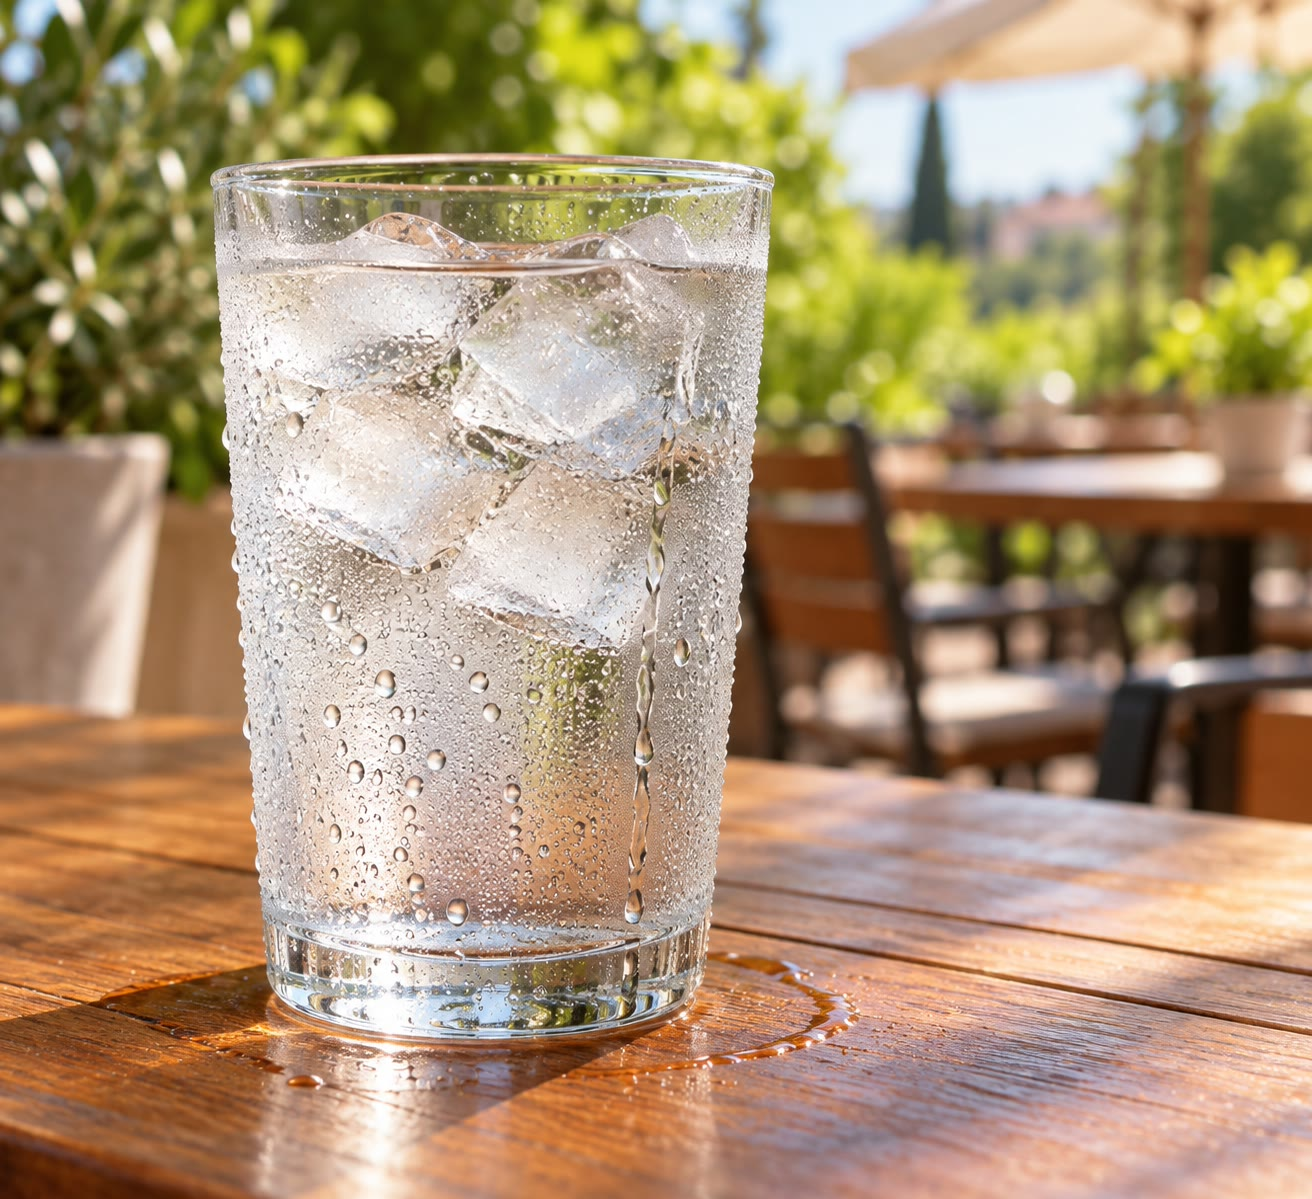
\includegraphics[width=0.5\linewidth]{images/book2/ai/g10-cold-glass.jpg}

{\small गर्मियों में छत पर बर्फ़ीले पानी का गिलास: उसके बाहरी भाग पर बूँदें बनती हैं, जहाँ
गिलास को छूती हवा ठंडी होती है।}
\end{omfigure}

\begin{recall}
बादल पानी की नन्ही बूँदों या बर्फ़ के क्रिस्टलों से बने होते हैं; उन्हें उनके आकार और ऊँचाई
के अनुसार कुलों में बाँटा जाता है, और वे वर्षा, हिम और ओले देते हैं, जिन्हें वर्षामापी से
मापा जाता है (पुस्तक 1, कक्षा 4)। वायुमंडल की सबसे निचली परत में हवा का तापमान ऊँचाई के
साथ घटता है, औसतन लगभग \qty{6.5}{\degreeCelsius} प्रति किलोमीटर; यह
पर्यावरणीय ह्रास दर है, और वाताग्र अलग-अलग तापमान की वायु राशियों को अलग करते हैं
(पुस्तक 1, कक्षा 8)। दाब ऊँचाई के साथ घटता है (भौतिकी की
पुस्तकें)। जल वाष्पित और संघनित होता है, और वाष्पन जो \omterm{def:g10:earth-energy-budget:latent-heat}{गुप्त ऊष्मा} अवशोषित करता है उसे
संघनन लौटा देता है (भौतिकी की पुस्तकें और
\cref{ch:g10:earth-energy-budget})।
\end{recall}
% ledger: nasa:grc-atmosphere

\section{जलवाष्प और संतृप्ति}

हवा में हमेशा कुछ जलवाष्प होती है, जो एक अदृश्य गैस है। वह कितनी जलवाष्प धारण कर
सकती है, यह सबसे बढ़कर उसके तापमान पर निर्भर करता है।

\begin{definition}[संतृप्ति; सापेक्ष आर्द्रता]\label{def:g10:why-clouds-form:humidity}
हवा \emph{संतृप्त}\index{संतृप्ति} होती है जब उसमें जलवाष्प का उतना सबसे बड़ा द्रव्यमान हो
जितना वह अपने तापमान पर धारण कर सकती है, यानी उसकी \emph{संतृप्ति
मात्रा}; कोई भी अतिरिक्त वाष्प संघनित होकर बूँदें बन जाती है। हवा की \emph{सापेक्ष
आर्द्रता}\index{सापेक्ष आर्द्रता} उसकी जलवाष्प की मात्रा को उसी तापमान और दाब पर उसकी
संतृप्ति मात्रा से भाग देकर मिलती है, और प्रतिशत में व्यक्त की जाती
है।
\end{definition}

यहाँ हवा में जल की मात्रा प्रति किलोग्राम शुष्क हवा में वाष्प के ग्राम में
(\unit{g/kg}) मापी जाती है: बिना जल पाए या खोए ऊपर उठने या नीचे बैठने वाला हवा का पार्सल
फैलने पर भी उतनी ही मात्रा रखता है।

\begin{omfigure}
\begin{tikzpicture}
\begin{axis}[omrecord, width=0.88\linewidth, height=6.2cm, xmin=-10, xmax=40,
  ymin=0, ymax=50, xlabel={तापमान (\unit{\degreeCelsius})},
  ylabel={संतृप्ति मात्रा (\unit{g/kg})}, xtick={-10,0,...,40},
  tick label style={font=\small}, label style={font=\small}]
\addplot[omDef!85!black, thick] table[x=T_C, y=ws_gkg] {figdata/out/grade-10-clouds-sat.dat};
\addplot[only marks, mark=*, mark size=1.8pt, omThm!85!black] coordinates {(28,11.37)};
\addplot[only marks, mark=o, mark size=1.8pt, omThm!85!black] coordinates {(16,11.37)};
\draw[->, omThm!85!black, thick] (axis cs:27.2,11.37) -- (axis cs:16.9,11.37);
\node[anchor=north, font=\footnotesize, omThm!85!black] at (axis cs:28,10.6) {\qty{28}{\degreeCelsius} पर हवा};
\node[anchor=south east, font=\footnotesize, omThm!85!black] at (axis cs:15.5,12.2) {ओसांक};
\node[anchor=south east, font=\footnotesize, omDef!85!black, align=right] at (axis cs:31,34) {वक्र के ऊपर:\\वाष्प संघनित होती है};
\node[anchor=south west, font=\footnotesize, omDef!85!black] at (axis cs:31,2.5) {असंतृप्त};
\node[anchor=north west, font=\footnotesize, omDef!85!black] at (axis cs:34,31.5) {संतृप्ति};
\end{axis}
\end{tikzpicture}

{\small एक किलोग्राम हवा जलवाष्प का जितना सबसे बड़ा द्रव्यमान धारण कर सकती है, वह
तापमान के सापेक्ष, समुद्र तल के दाब पर (द्रव जल के ऊपर; जल के अंतरराष्ट्रीय मानक से
परिकलित)। \qty{28}{\degreeCelsius} पर
\qty{11.4}{g/kg} धारण करने वाली हवा (बिंदु) \omterm{def:g10:why-clouds-form:humidity}{संतृप्ति} से बहुत दूर है; बिना जल खोए ठंडी होने
पर वह \qty{16}{\degreeCelsius} पर \omterm{def:g10:why-clouds-form:humidity}{संतृप्त} हो जाती है (वृत्त)।}
\end{omfigure}
% ledger: iapws:vapour-pressure, ciaaw:abridged-2024, earth:Mmol, const:R (computed in figdata/grade-10/clouds.py)

वक्र तेज़ी से चढ़ता है: \qty{0}{\degreeCelsius} पर \qty{3.8}{g/kg},
\qty{20}{\degreeCelsius} पर \qty{14.7}{g/kg}, \qty{30}{\degreeCelsius} पर
\qty{27.2}{g/kg}। हर \qty{10}{\degreeCelsius} की तापवृद्धि हवा द्वारा धारण किए जा सकने वाले
जल को लगभग दुगुना कर देती है। इसी कारण उष्णकटिबंधीय हवा मूसलाधार वर्षा ला सकती है, और
ध्रुवीय सर्दी की हवा, \omterm{def:g10:why-clouds-form:humidity}{संतृप्त} होने पर भी, लगभग कुछ भी धारण नहीं करती।

\begin{definition}[ओसांक]\label{def:g10:why-clouds-form:dew-point}
हवा का \emph{ओसांक}\index{ओसांक} वह तापमान है जिस तक उसे, उसकी जल-मात्रा और दाब
बनाए रखते हुए, ठंडा करना पड़ता है ताकि वह
\omterm{def:g10:why-clouds-form:humidity}{संतृप्त} हो जाए।
\end{definition}

\begin{method}[तालिका से सापेक्ष आर्द्रता और ओसांक]\label{met:g10:why-clouds-form:table}
\begin{enumerate}
  \item तालिका में हवा के तापमान पर \omterm{def:g10:why-clouds-form:humidity}{संतृप्ति} मात्रा पढ़िए।
  \item \omterm{def:g10:why-clouds-form:humidity}{सापेक्ष आर्द्रता}: हवा की जल-मात्रा को उससे भाग दीजिए।
  \item \omterm{def:g10:why-clouds-form:dew-point}{ओसांक}: तालिका में वह तापमान खोजिए जिसकी \omterm{def:g10:why-clouds-form:humidity}{संतृप्ति}
        मात्रा हवा की जल-मात्रा के बराबर है।
\end{enumerate}
\end{method}

\begin{example}[गर्मियों की एक सुबह]\label{ex:g10:why-clouds-form:morning}
% ledger: iapws:vapour-pressure (values computed in figdata/grade-10/clouds.py)
\qty{20}{\degreeCelsius} पर हवा में \qty{11.4}{g/kg} है।
\qty{20}{\degreeCelsius} पर \omterm{def:g10:why-clouds-form:humidity}{संतृप्ति} मात्रा \qty{14.7}{g/kg} है, इसलिए
\omterm{def:g10:why-clouds-form:humidity}{सापेक्ष आर्द्रता} $11.4/14.7 \approx \qty{78}{\percent}$ है। \omterm{def:g10:why-clouds-form:humidity}{संतृप्ति}
मात्रा \qty{16}{\degreeCelsius} पर \qty{11.4}{g/kg} है: यही \omterm{def:g10:why-clouds-form:dew-point}{ओसांक}
है। दोपहर में वही हवा \qty{28}{\degreeCelsius} तक गरम होकर
(\omterm{def:g10:why-clouds-form:humidity}{संतृप्ति} मात्रा \qty{24.1}{g/kg}) केवल
\qty{47}{\percent} की \omterm{def:g10:why-clouds-form:humidity}{सापेक्ष आर्द्रता} रखती है --- उसमें ठीक उतना ही जल होते हुए।
\end{example}

आरंभ का गिलास अपने आसपास की हवा के \omterm{def:g10:why-clouds-form:dew-point}{ओसांक} से अधिक ठंडा है: उसे छूने वाली हवा अपने
\omterm{def:g10:why-clouds-form:dew-point}{ओसांक} से नीचे ठंडी हो जाती है और गिलास पर जल छोड़ देती है। साफ़ रात में घास और कारों की
छतें आकाश की ओर अवरक्त विकिरित करके ऊष्मा खोती हैं और हवा से अधिक ठंडी हो जाती हैं:
उन पर ओस बनती है, या \qty{0}{\degreeCelsius} से नीचे पाला। जब ज़मीन के पास हवा की पूरी
परत अपने \omterm{def:g10:why-clouds-form:dew-point}{ओसांक} तक ठंडी हो जाती है, तो बूँदें हवा में ही बनती हैं: कोहरा।

\begin{omfigure}
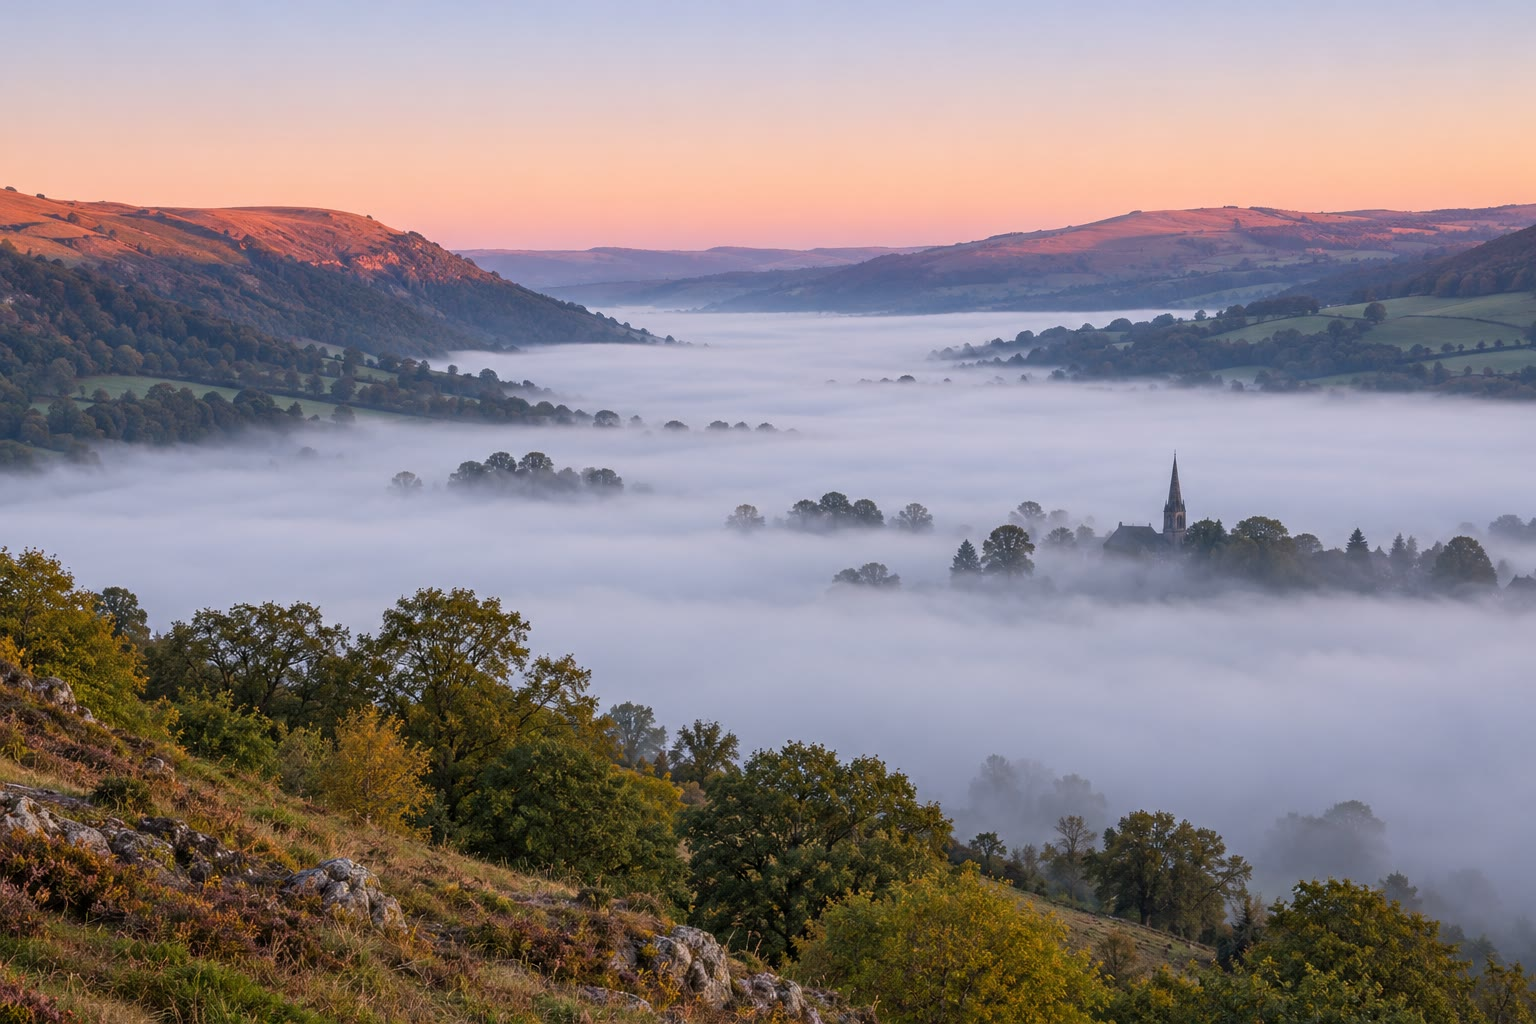
\includegraphics[width=0.75\linewidth]{images/book2/ai/g10-valley-fog.jpg}

{\small भोर में एक घाटी को भरता कोहरा। साफ़ रात में ज़मीन ठंडी हुई, ठंडी हवा बहकर
घाटी में नीचे उतरी, और वहाँ वह अपने \omterm{def:g10:why-clouds-form:dew-point}{ओसांक} से नीचे
ठंडी हो गई।}
\end{omfigure}

\section{ऊपर उठती हवा ठंडी होती है}

अधिकांश बादल इसलिए नहीं बनते कि हवा किसी ठंडी चीज़ को छूती है। वे इसलिए बनते हैं
कि हवा ऊपर उठती है। दाब ऊँचाई के साथ घटता है; ऊपर उठता हवा का पार्सल
फैलता है, आसपास की हवा को पीछे धकेलता है, और इस कार्य के लिए ऊर्जा
स्वयं पार्सल से ली जाती है।

\begin{definition}[रुद्धोष्म शीतलन; शुष्क रुद्धोष्म दर]\label{def:g10:why-clouds-form:adiabatic}
\emph{रुद्धोष्म शीतलन}\index{रुद्धोष्म शीतलन} हवा के ऐसे पार्सल का शीतलन है जो
अपने परिवेश से ऊष्मा का आदान-प्रदान किए बिना फैलता है।
ऊपर उठती असंतृप्त हवा जिस दर से इस प्रकार ठंडी होती है, वह \emph{शुष्क
रुद्धोष्म दर}\index{शुष्क रुद्धोष्म दर} है, जो आरोहण के प्रति किलोमीटर
\qty{9.8}{\degreeCelsius} के निकट है; नीचे बैठती हवा उसी दर से
गरम होती है।
\end{definition}

\begin{proposition}[शुष्क रुद्धोष्म दर]\label{prop:g10:why-clouds-form:dry-rate}
\omterm{def:g10:why-clouds-form:adiabatic}{शुष्क रुद्धोष्म दर} $g/c_p$ है, जहाँ $g = \qty{9.81}{m/s^2}$ और $c_p
\approx \qty{1005}{J.kg^{-1}.K^{-1}}$ वह ऊर्जा है जो \omterm{def:g10:why-clouds-form:stability}{स्थिर} दाब पर एक किलोग्राम
हवा को एक अंश गरम करती है: $9.81/1005 \approx
\qty{0.0098}{\degreeCelsius/m}$, यानी \qty{9.8}{\degreeCelsius/km}।
(स्वीकृत: इसकी उपपत्ति भौतिकी की पुस्तकों का विषय है।)
\end{proposition}
% ledger: const:gn, const:R, earth:Mmol (c_p of dry air computed as (7/2)R/M in figdata/grade-10/clouds.py)

ऊपर उठने पर पार्सल का \omterm{def:g10:why-clouds-form:dew-point}{ओसांक} भी घटता है, पर धीरे: उसकी जल-मात्रा
वही रहती है, जबकि दाब की गिरावट वाष्प को \omterm{def:g10:why-clouds-form:humidity}{संतृप्त} करना थोड़ा आसान बना देती है।
ज़मीन के पास की हवा के लिए परिकलन लगभग
\qty{1.8}{\degreeCelsius} प्रति किलोमीटर देता है। इसलिए पार्सल का तापमान अपने \omterm{def:g10:why-clouds-form:dew-point}{ओसांक} की
ओर हर किलोमीटर की चढ़ाई में लगभग $9.8 - 1.8 = \qty{8}{\degreeCelsius}$
पास आता जाता है।
% ledger: iapws:vapour-pressure (dew-point rate computed in figdata/grade-10/clouds.py)

\begin{definition}[संघनन तल]\label{def:g10:why-clouds-form:condensation-level}
हवा के किसी पार्सल का \emph{संघनन तल}\index{संघनन तल} वह ऊँचाई है जिस पर ऊपर उठते
हुए वह \omterm{def:g10:why-clouds-form:humidity}{संतृप्त} हो जाता है। उसके ऊपर जल संघनित होता है:
संघनन तल ऊपर उठती हवा से बनने वाले बादलों का चपटा
आधार है।
\end{definition}

\begin{proposition}[संघनन तल की ऊँचाई]\label{prop:g10:why-clouds-form:lcl}
तापमान $T$ और \omterm{def:g10:why-clouds-form:dew-point}{ओसांक} $T_d$
(\unit{\degreeCelsius} में) के साथ ज़मीन से उठने वाली हवा लगभग इस ऊँचाई पर \omterm{def:g10:why-clouds-form:humidity}{संतृप्त} होती है:
\[
  z = \frac{T - T_d}{8}\ \text{km} = \qty{125}{m} \times (T - T_d).
\]
\end{proposition}

\begin{proof}
ऊँचाई $z$ (km में) पर पार्सल का तापमान $T - 9.8\,z$ है और उसका
\omterm{def:g10:why-clouds-form:dew-point}{ओसांक} $T_d - 1.8\,z$। जब ये बराबर हों तब वह \omterm{def:g10:why-clouds-form:humidity}{संतृप्त} होता है:
$T - 9.8\,z = T_d - 1.8\,z$, इसलिए $8\,z = T - T_d$ और $z = (T - T_d)/8$ km।
एक किलोमीटर का आठवाँ भाग \qty{125}{m} है।
\end{proof}

\begin{example}[दोपहर का एक कपासी मेघ]\label{ex:g10:why-clouds-form:base}
% ledger: iapws:vapour-pressure (exact ascent computed in figdata/grade-10/clouds.py: 1.51 km)
\cref{ex:g10:why-clouds-form:morning} की दोपहर में ज़मीन पर हवा
\qty{28}{\degreeCelsius} पर है और उसका \omterm{def:g10:why-clouds-form:dew-point}{ओसांक}
\qty{16}{\degreeCelsius}। ऊपर उठते बुलबुले
$125 \times 12 = \qty{1500}{m}$ पर \omterm{def:g10:why-clouds-form:humidity}{संतृप्त} होते हैं: कपासी मेघों के चपटे आधार लगभग
\qty{1.5}{km} ऊपर हैं। सुबह, \qty{20}{\degreeCelsius} पर, यही हवा
केवल $125 \times 4 = \qty{500}{m}$ पर संघनित हो जाती: ज़मीन के गरम होने के साथ दिन भर
बादलों के आधार ऊपर उठते जाते हैं।
\end{example}

\section{स्थिर और अस्थिर वायु}

ऊपर उठता पार्सल ऊपर उठता रहेगा या नहीं, यह उसके आसपास की हवा पर निर्भर करता है। अपने
परिवेश से अधिक गरम पार्सल अपने द्वारा हटाई गई हवा से हल्का होता है और ऊपर उठता है,
गरम हवा के गुब्बारे की तरह; अपने परिवेश से अधिक ठंडा पार्सल वापस नीचे बैठ जाता है।

\begin{definition}[स्थिर वायु; अस्थिर वायु]\label{def:g10:why-clouds-form:stability}
वायु \emph{स्थिर}\index{स्थिर वायु} होती है जब ऊपर धकेला गया पार्सल अपने आसपास की हवा से
अधिक ठंडा हो जाता है, और इसलिए वापस वहीं बैठ जाता है जहाँ से चला था। वह
\emph{अस्थिर}\index{अस्थिर वायु} होती है जब पार्सल अपने आसपास की हवा से अधिक गरम हो
जाता है और अपने आप ऊपर उठता रहता है।
\end{definition}

ऊपर उठता पार्सल, जब तक \omterm{def:g10:why-clouds-form:humidity}{संतृप्त} न हो, \omterm{def:g10:why-clouds-form:adiabatic}{शुष्क रुद्धोष्म दर}, \qty{9.8}{\degreeCelsius}
प्रति किलोमीटर, से ठंडा होता है। \omterm{def:g10:why-clouds-form:humidity}{संतृप्त} होने के बाद वह
अधिक धीरे ठंडा होता है: संघनन पार्सल में \omterm{def:g10:earth-energy-budget:latent-heat}{गुप्त ऊष्मा} छोड़ता है। परिकलन
ज़मीन के पास की गरम हवा में लगभग \qty{4.7}{\degreeCelsius} प्रति किलोमीटर,
\qty{0}{\degreeCelsius} पर लगभग \num{5.8}, और ऊपर की ठंडी हवा में, जहाँ संघनित
होने के लिए थोड़ा ही जल बचता है, इससे अधिक देता है; यह
\omterm{def:g10:why-clouds-form:humidity}{संतृप्त} दर है। (इसका सूत्र विश्वविद्यालय के खंडों में निकाला गया है।)
% ledger: nist:water-latent, iapws:vapour-pressure (saturated rates computed in figdata/grade-10/clouds.py)

\begin{method}[क्या यह वायु स्थिर है?]\label{met:g10:why-clouds-form:stable}
\begin{enumerate}
  \item पता कीजिए कि आसपास की हवा का तापमान ऊँचाई के साथ कितनी तेज़ी से घटता है
        (पर्यावरणीय ह्रास दर, गुब्बारे के परिज्ञापन से)।
  \item इसकी तुलना उस दर से कीजिए जिससे पार्सल ठंडा होता है: अपने \omterm{def:g10:why-clouds-form:condensation-level}{संघनन तल} के नीचे
        शुष्क दर, लगभग \qty{9.8}{\degreeCelsius/km};
        उसके ऊपर \omterm{def:g10:why-clouds-form:humidity}{संतृप्त} दर, लगभग \qty{5}{\degreeCelsius/km}।
  \item यदि परिवेश पार्सल से धीरे ठंडा होता है, तो पार्सल अंत में
        अधिक ठंडा रहता है: \omterm{def:g10:why-clouds-form:stability}{स्थिर}। यदि परिवेश तेज़ी से ठंडा होता है, तो पार्सल अंत में
        अधिक गरम रहता है: \omterm{def:g10:why-clouds-form:stability}{अस्थिर}। जिस परत में ऊँचाई के साथ तापमान \emph{बढ़ता} है वह
        बहुत \omterm{def:g10:why-clouds-form:stability}{स्थिर} होती है: वह ऊपर उठती हवा को ढक्कन की तरह रोक देती है।
\end{enumerate}
\end{method}

लगभग \qty{6.5}{\degreeCelsius/km} की औसत ह्रास दर के साथ वायु तब तक \omterm{def:g10:why-clouds-form:stability}{स्थिर} है
जब तक वह असंतृप्त है (पार्सल अधिक तेज़ी से ठंडा होता है) और \omterm{def:g10:why-clouds-form:humidity}{संतृप्त} होते ही \omterm{def:g10:why-clouds-form:stability}{अस्थिर}
(पार्सल अधिक धीरे ठंडा होता है)। ऐसी वायु को
सशर्त \omterm{def:g10:why-clouds-form:stability}{अस्थिर} कहा जाता है: वह \omterm{def:g10:why-clouds-form:stability}{स्थिर} रहती है जब तक कोई चीज़ उसे
उसके \omterm{def:g10:why-clouds-form:condensation-level}{संघनन तल} तक न उठा दे, और फिर बादल अपने आप बढ़ता है।

\begin{omfigure}
\begin{tikzpicture}
\begin{axis}[omrecord, width=0.9\linewidth, height=7.6cm, xmin=-30, xmax=36,
  ymin=0, ymax=6, xlabel={तापमान (\unit{\degreeCelsius})}, ylabel={ऊँचाई (km)},
  xtick={-30,-20,...,30}, ytick={0,1,...,6},
  legend style={at={(0.02,0.98)}, anchor=north west, font=\footnotesize, draw=black!30, fill=white},
  tick label style={font=\small}, label style={font=\small}]
\fill[omDef!10] (axis cs:-30,1.51) rectangle (axis cs:36,3.96);
\addplot[black!60, thick] table[x=T_C, y=z_km] {figdata/out/grade-10-clouds-envA.dat};
\addlegendentry{परिज्ञापन A}
\addplot[omProp!90!black, thick, densely dotted] table[x=T_C, y=z_km] {figdata/out/grade-10-clouds-envB.dat};
\addlegendentry{परिज्ञापन B}
\addplot[omThm!85!black, very thick] table[x=T_C, y=z_km] {figdata/out/grade-10-clouds-parcel.dat};
\addlegendentry{ऊपर उठता पार्सल}
\addplot[omMeth!85!black, thick, dashed] table[x=Td_C, y=z_km] {figdata/out/grade-10-clouds-dew.dat};
\addlegendentry{उसका ओसांक}
\draw[black!50, dashed] (axis cs:-30,1.51) -- (axis cs:36,1.51);
\node[anchor=south west, font=\footnotesize] at (axis cs:-29.5,1.53) {संघनन तल};
\node[anchor=north east, font=\footnotesize, omDef!80!black] at (axis cs:35.5,3.9) {A के साथ बादल};
\end{axis}
\end{tikzpicture}

{\small \qty{28}{\degreeCelsius} पर और \qty{16}{\degreeCelsius} के
\omterm{def:g10:why-clouds-form:dew-point}{ओसांक} के साथ ज़मीन से उठता एक पार्सल (परिकलित): वह शुष्क दर से ठंडा होता है
जब तक \qty{1.5}{km} पर उसका तापमान उसके \omterm{def:g10:why-clouds-form:dew-point}{ओसांक} से नहीं मिल जाता, फिर
धीमी \omterm{def:g10:why-clouds-form:humidity}{संतृप्त} दर से। दो कल्पित परिज्ञापन: A में पार्सल
\qty{1.5}{km} से लेकर लगभग \qty{4}{km} की गरम परत तक अपने परिवेश से अधिक गरम
है, और इनके बीच एक कपासी मेघ बढ़ता है (छायांकित); B में ज़मीन के ऊपर की गरम
हवा पार्सल को हर जगह उसके परिवेश से अधिक ठंडा रखती है:
\omterm{def:g10:why-clouds-form:stability}{स्थिर वायु}, कोई कपासी मेघ नहीं।}
\end{omfigure}
% ledger: iapws:vapour-pressure, nist:water-latent (parcel computed in figdata/grade-10/clouds.py; soundings invented)

जब वायु \omterm{def:g10:why-clouds-form:stability}{स्थिर} हो और फिर भी उठाई जाए --- किसी पर्वत के ऊपर, या
किसी वाताग्र के अनुदिश --- तो बनने वाले बादल चपटी धूसर परतों में फैल जाते हैं:
स्तरी मेघ। जब वह \omterm{def:g10:why-clouds-form:stability}{अस्थिर} हो, तो बादल ढेरों में ऊपर की ओर उमड़ते हैं: कपासी मेघ,
और, जब अस्थिरता काफ़ी ऊँचाई तक पहुँचे, तड़ित-झंझाओं के कपासी वर्षी मेघ, जिनके
शीर्ष वायुमंडल की सबसे निचली परत के ऊपर की बहुत \omterm{def:g10:why-clouds-form:stability}{स्थिर} हवा से मिलने पर निहाई के आकार में
फैल जाते हैं।

\begin{omfigure}
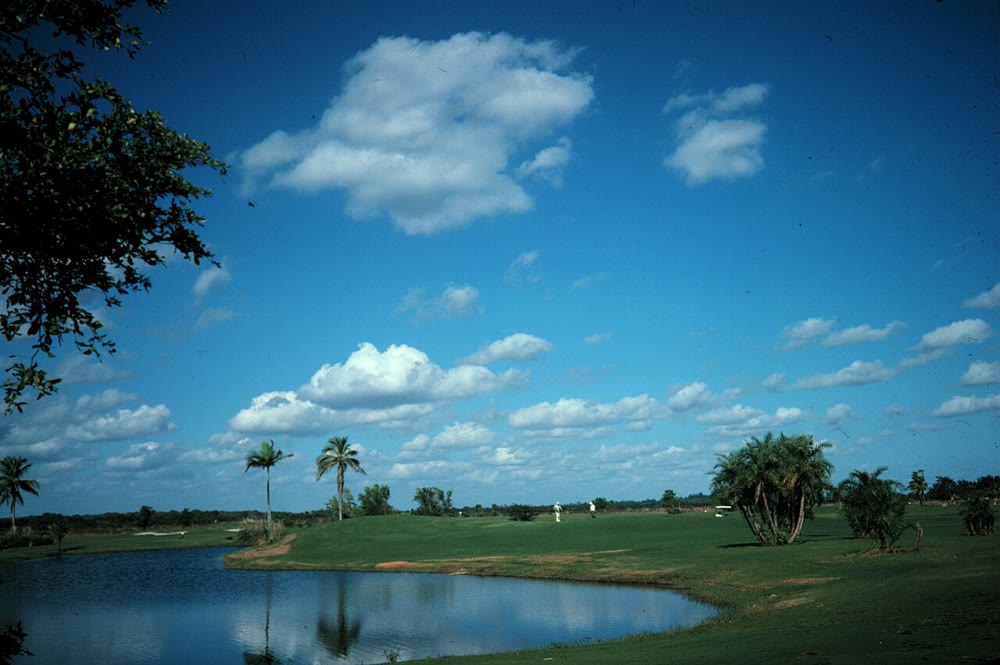
\includegraphics[height=4.5cm]{images/book2/g10-noaa-fair-weather-cumulus.jpg}\hspace{0.6em}%
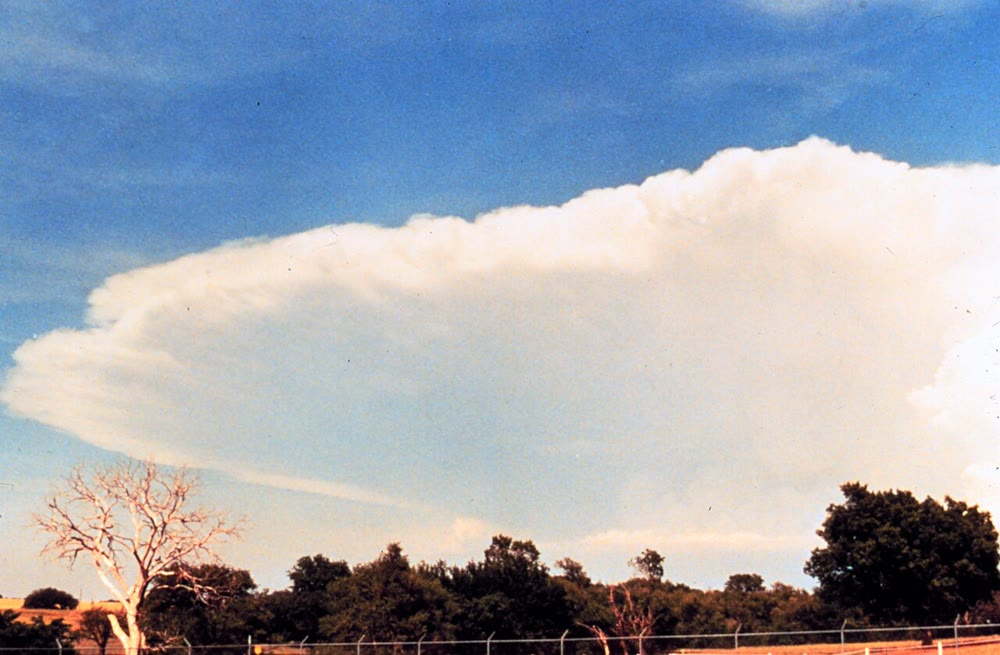
\includegraphics[height=4.5cm]{images/book2/g10-noaa-cumulonimbus-anvil.jpg}

{\small बाएँ: फ़्लोरिडा के ऊपर साफ़ मौसम के कपासी मेघ, जिनके चपटे आधार उनके
\omterm{def:g10:why-clouds-form:condensation-level}{संघनन तल} पर हैं। फ़ोटो: राल्फ़ एफ़॰ क्रेस्गे, NOAA (सार्वजनिक डोमेन)।
दाएँ: तूफ़ान की आरंभिक अवस्था में कपासी वर्षी मेघ की निहाई।
फ़ोटो: NOAA की राष्ट्रीय प्रचंड तूफ़ान प्रयोगशाला (सार्वजनिक डोमेन)।}
\end{omfigure}

\section{हवा को उठाने के चार तरीक़े}

हवा चार कारणों से ऊपर उठती है।
\begin{itemize}
  \item \textbf{नीचे से गरम होना।} धूप वाले दिन ज़मीन अपने ऊपर की हवा को गरम करती है;
        सबसे गरम हिस्सों से गरम हवा के बुलबुले ऊपर उठते हैं। इन्हीं से दोपहर के
        कपासी मेघ बनते हैं।
  \item \textbf{पर्वत।} किसी पर्वत-श्रेणी से टकराती पवन उसकी ढलान पर ऊपर चढ़ने को
        विवश होती है।
  \item \textbf{वाताग्र।} जहाँ गरम और ठंडी वायु राशियाँ मिलती हैं, वहाँ हल्की गरम
        हवा ठंडी हवा के ऊपर चढ़ती है, या ठंडी हवा उसके नीचे घुस जाती है (पुस्तक 1,
        कक्षा 8)।
  \item \textbf{अभिसरण।} जब ज़मीन के पास पवनें एक साथ बहकर मिलती हैं, तो हवा के पास
        ऊपर जाने के सिवा कोई रास्ता नहीं बचता, जैसे भूमध्य रेखा के पास ऊपर उठती हवा की
        पट्टी में और किसी अवदाब के केंद्र में।
\end{itemize}

\begin{method}[पर्वत के ऊपर से किसी पार्सल का अनुसरण]\label{met:g10:why-clouds-form:mountain}
\begin{enumerate}
  \item 125-मीटर नियम से \omterm{def:g10:why-clouds-form:condensation-level}{संघनन तल} ज्ञात कीजिए; वहाँ तक
        पार्सल \qty{9.8}{\degreeCelsius/km} से ठंडा होता है।
  \item वहाँ से शिखर तक वह \omterm{def:g10:why-clouds-form:humidity}{संतृप्त} दर से ठंडा होता है; संघनित होने वाला जल
        पवनाभिमुख ढाल पर वर्षा या हिम के रूप में गिरता है।
  \item शिखर के पार पार्सल असंतृप्त होकर नीचे उतरता है: वह पूरे रास्ते
        \qty{9.8}{\degreeCelsius/km} से गरम होता है।
\end{enumerate}
\end{method}

\begin{example}[अनुवात ढाल की गरम शुष्क पवन]\label{ex:g10:why-clouds-form:lee}
% ledger: iapws:vapour-pressure, nist:water-latent (all values computed in figdata/grade-10/clouds.py)
समुद्र तल पर \qty{20}{\degreeCelsius} की हवा, जिसका \omterm{def:g10:why-clouds-form:dew-point}{ओसांक}
\qty{12}{\degreeCelsius} है, \qty{2500}{m} ऊँचे एक कटक के ऊपर से धकेली जाती है। वह
$125 \times 8 = \qty{1000}{m}$ पर, लगभग
\qty{10}{\degreeCelsius} पर, \omterm{def:g10:why-clouds-form:humidity}{संतृप्त} हो जाती है। वहाँ से शिखर तक वह \omterm{def:g10:why-clouds-form:humidity}{संतृप्त}
दर से ठंडी होती है, लगभग \qty{2}{\degreeCelsius} तक, और अपने जल का लगभग एक-तिहाई वर्षा
के रूप में खो देती है (\num{8.7} से \qty{6.0}{g/kg})। दूसरी ओर नीचे उतरते हुए
वह \qty{2.5}{km} तक शुष्क दर से गरम होती है: वह मैदान पर लगभग
\qty{27}{\degreeCelsius} पर पहुँचती है, जहाँ से चली थी उससे सात अंश अधिक गरम, और
उसकी \omterm{def:g10:why-clouds-form:humidity}{सापेक्ष आर्द्रता} लगभग \qty{27}{\percent} होती है। ऐसी गरम, शुष्क पवनें
अनेक पर्वत-श्रेणियों के अनुवात ढाल पर चलती हैं।
\end{example}

\begin{omfigure}
\begin{tikzpicture}[font=\footnotesize, >={Stealth[length=2mm]}]
  \fill[omExo!30] (0,0) -- (3.5,0.3) -- (6,3.0) -- (8.5,0.3) -- (12,0) -- (12,-0.25) -- (0,-0.25) -- cycle;
  \draw[thick, black!70] (0,0) -- (3.5,0.3) -- (6,3.0) -- (8.5,0.3) -- (12,0);
  \draw[black!40, dashed] (0,1.2) -- (4.6,1.2);
  \node[anchor=south west, black!60, align=left] at (0.1,1.22) {संघनन\\तल, \qty{1000}{m}};
  \foreach \x in {3.62,3.86,4.1} \draw[omDef!60] (\x,1.2) -- (\x-0.06,{0.3+(\x-0.06-3.5)*1.08+0.04});
  \pic[scale=1.1, transform shape] at (4.6,1.22) {puffycloud};
  \pic[scale=0.9, transform shape] at (5.0,2.2) {puffycloud};
  \draw[->, thick, omDef!80!black] (0.2,0.25) -- (2.8,0.5) .. controls (3.6,0.75) .. (4.4,1.7) -- (5.4,2.9) .. controls (5.8,3.4) and (6.2,3.4) .. (6.6,2.9) -- (7.6,1.7) .. controls (8.4,0.75) .. (9.2,0.5) -- (11.8,0.25);
  \node[anchor=east, align=right] at (3.4,2.15) {\qty{10}{\degreeCelsius}, संतृप्त};
  \node[anchor=south, align=center] at (6.0,3.45) {शिखर \qty{2500}{m}: \qty{2}{\degreeCelsius}};
  \node[anchor=west, align=left] at (7.75,2.1) {नीचे उतरती और\\\qty{9.8}{\degreeCelsius/km} से गरम होती};
  \node[anchor=north, align=center] at (1.0,-0.3) {\qty{20}{\degreeCelsius}\\ओसांक \qty{12}{\degreeCelsius}};
  \node[anchor=north, align=center] at (11.0,-0.3) {\qty{27}{\degreeCelsius}\\ओसांक \qty{6}{\degreeCelsius}};
  \node[anchor=north, black!60] at (4.0,-0.3) {पवनाभिमुख: वर्षा};
  \node[anchor=north, black!60] at (8.2,-0.3) {अनुवात: शुष्क};
\end{tikzpicture}

{\small पर्वत के एक कटक को पार करता हवा का पार्सल (तापमान परिकलित;
ऊर्ध्वाधर पैमाना बढ़ाया गया)। वह अपने \omterm{def:g10:why-clouds-form:condensation-level}{संघनन तल} तक शुष्क दर से ठंडा होता है,
उसके ऊपर धीमी \omterm{def:g10:why-clouds-form:humidity}{संतृप्त} दर से, वर्षा के रूप में जल खोते हुए, और अनुवात ढाल पर
पूरे रास्ते शुष्क दर से गरम होता है।}
\end{omfigure}

\section{बूँदों से वर्षा और हिम तक}

बिल्कुल स्वच्छ हवा में जलवाष्प आसानी से संघनित नहीं होती। बूँदें पदार्थ के कणों पर
बनती हैं।

\begin{definition}[संघनन केंद्रक]\label{def:g10:why-clouds-form:nucleus}
\emph{संघनन केंद्रक}\index{संघनन केंद्रक} हवा में निलंबित एक नन्हा कण है --- समुद्री
नमक, धूल, धुएँ या कालिख का एक कण --- जिस पर जलवाष्प संघनित होकर बादल की एक बूँद
बनाती है।
\end{definition}

एक सामान्य केंद्रक लगभग \qty{0.0002}{mm} का होता है, बादल की एक बूँद लगभग
\qty{0.02}{mm} की, फुहार की एक बूँद \qty{0.5}{mm} की और वर्षा की एक बूँद लगभग
\qty{2}{mm} की। वर्षा की बूँद बादल की बूँद से सौ गुना चौड़ी होती है, इसलिए उसका
आयतन $100^3$ गुना बड़ा होता है: बादल की एक मिलियन बूँदें मिलकर वर्षा की एक बूँद बनाती हैं।
बादल की बूँदें इतनी छोटी होती हैं कि हल्की-सी ऊर्ध्व धारा भी उन्हें
ऊपर टिकाए रखती है; वर्षा गिरने के लिए बूँदों को सौ गुना बढ़ना पड़ता है।
% ledger: jpl:drop-sizes

\begin{omfigure}
\begin{tikzpicture}
\begin{axis}[width=0.9\linewidth, height=3.4cm, xmode=log, xmin=1e-4, xmax=10,
  ymin=0, ymax=1, axis y line=none, axis x line*=bottom,
  xlabel={व्यास (mm), लघुगणकीय पैमाना}, tick label style={font=\small},
  label style={font=\small}, clip=false]
\addplot[only marks, mark=*, omDef!85!black, mark size=2.5pt] coordinates {(0.0002,0.3) (0.02,0.3) (0.5,0.3) (2,0.3)};
\node[anchor=south, font=\footnotesize, align=center] at (axis cs:0.0002,0.42) {संघनन\\केंद्रक};
\node[anchor=south, font=\footnotesize, align=center] at (axis cs:0.02,0.42) {बादल की\\बूँद};
\node[anchor=south, font=\footnotesize, align=center] at (axis cs:0.5,0.42) {फुहार};
\node[anchor=south, font=\footnotesize, align=center] at (axis cs:2,0.42) {वर्षा की\\बूँद};
\end{axis}
\end{tikzpicture}

{\small सामान्य आकार, ऐसे पैमाने पर जहाँ हर चरण पिछले का दस गुना है: फुहार को छोड़कर
हर वस्तु पिछली वस्तु से लगभग सौ गुना चौड़ी है। आँकड़े: NASA जेट प्रणोदन
प्रयोगशाला।}
\end{omfigure}

दो प्रक्रम उन्हें बढ़ाते हैं।

\begin{definition}[उष्ण-वर्षा प्रक्रम; हिम-क्रिस्टल प्रक्रम]\label{def:g10:why-clouds-form:rain-processes}
\emph{उष्ण-वर्षा प्रक्रम}\index{उष्ण-वर्षा प्रक्रम} में बादल की बड़ी
बूँदें छोटी बूँदों से तेज़ गिरती हैं, उनसे टकराकर
मिल जाती हैं, और गिरते हुए बढ़ती जाती हैं। \emph{हिम-क्रिस्टल
प्रक्रम}\index{हिम-क्रिस्टल प्रक्रम} में, बादल के उस भाग में जो
\qty{0}{\degreeCelsius} से ठंडा है और जहाँ बर्फ़ के क्रिस्टल और अतिशीतित बूँदें (जो
\qty{0}{\degreeCelsius} से नीचे भी द्रव हैं) मिली-जुली होती हैं, क्रिस्टल उस
वाष्प को लेकर बढ़ते हैं जिसे बूँदें वाष्पित करती हैं; वे हिमकणों के रूप में गिरते हैं, और नीचे की
हवा गरम हो तो पिघलकर वर्षा की बूँदें बन जाते हैं।
\end{definition}

\omterm{def:g10:why-clouds-form:rain-processes}{हिम-क्रिस्टल प्रक्रम} इसलिए काम करता है कि एक ही तापमान पर \omterm{def:g10:why-clouds-form:humidity}{संतृप्ति} मात्रा द्रव जल की
तुलना में बर्फ़ के ऊपर कम होती है:
\qty{-10}{\degreeCelsius} पर \omterm{def:g10:why-clouds-form:humidity}{संतृप्त} वाष्प दाब जल के ऊपर \qty{287}{Pa}
और बर्फ़ के ऊपर \qty{260}{Pa} है। बूँदों के लिए \omterm{def:g10:why-clouds-form:humidity}{संतृप्त} हवा उतनी वाष्प से
\qty{10}{\percent} अधिक धारण करती है जितनी बर्फ़ सह सकती है: वाष्प
क्रिस्टलों पर संघनित होती है, और उसकी पूर्ति के लिए बूँदें वाष्पित होती हैं।
% ledger: iapws:vapour-pressure, iapws:melt-subl (computed in figdata/grade-10/clouds.py)

\begin{remark}[गुप्त ऊष्मा तूफ़ान को पोषण देती है]\label{rem:g10:why-clouds-form:latent}
बादल में संघनित होने वाला हर किलोग्राम जल हवा को लगभग
\qty{2.5}{MJ} देता है, वही \omterm{def:g10:earth-energy-budget:latent-heat}{गुप्त ऊष्मा} जो वाष्पित होते समय समुद्र या ज़मीन से ली गई थी
(\cref{ch:g10:earth-energy-budget})। यही ऊष्मा \omterm{def:g10:why-clouds-form:humidity}{संतृप्त} दर को शुष्क दर से धीमा
बनाती है और कपासी वर्षी मेघ को ऊपर उठाए रखती है;
\cref{ch:g10:storms-and-cyclones} सबसे बड़े तूफ़ानों में उसका अनुसरण करता है।
\end{remark}
% ledger: nist:water-latent

\section{अभ्यास}

इन अभ्यासों के लिए नीचे की तालिका की \omterm{def:g10:why-clouds-form:humidity}{संतृप्ति} मात्राएँ (\unit{g/kg} में, समुद्र तल
के दाब पर), शुष्क दर
\qty{9.8}{\degreeCelsius/km}, \omterm{def:g10:why-clouds-form:dew-point}{ओसांक} की \qty{1.8}{\degreeCelsius/km} की गिरावट
और \qty{5}{\degreeCelsius/km} की \omterm{def:g10:why-clouds-form:humidity}{संतृप्त} दर लीजिए।
% ledger: iapws:vapour-pressure (table from figdata/out/grade-10-clouds-sat.dat, rounded)

\begin{center}
\small
\begin{tabular}{l*{11}{c}}
\hline
तापमान (\unit{\degreeCelsius}) & 0 & 4 & 8 & 10 & 12 & 14 & 16 & 20 & 24 & 28 & 30 \\
\omterm{def:g10:why-clouds-form:humidity}{संतृप्ति} मात्रा (\unit{g/kg}) & 3.8 & 5.0 & 6.7 & 7.6 & 8.7 & 10.0 & 11.4 & 14.7 & 18.9 & 24.1 & 27.2 \\
\hline
\end{tabular}
\end{center}

\begin{exercise}[$\star$]\label{exo:g10:why-clouds-form:1}
हवा की \omterm{def:g10:why-clouds-form:humidity}{सापेक्ष आर्द्रता} और \omterm{def:g10:why-clouds-form:dew-point}{ओसांक} की परिभाषा दीजिए।
\end{exercise}

\begin{exercise}[$\star$]\label{exo:g10:why-clouds-form:2}
तालिका से \num{0}, \num{10},
\num{20} और \qty{30}{\degreeCelsius} पर \omterm{def:g10:why-clouds-form:humidity}{संतृप्ति} मात्रा बताइए। हर \qty{10}{\degreeCelsius}
की तापवृद्धि पर यह मोटे तौर पर किस गुणक से बढ़ती है?
\end{exercise}

\begin{exercise}[$\star$]\label{exo:g10:why-clouds-form:3}
\qty{24}{\degreeCelsius} पर हवा में \qty{10.0}{g/kg} जलवाष्प है।
उसकी \omterm{def:g10:why-clouds-form:humidity}{सापेक्ष आर्द्रता} और उसका \omterm{def:g10:why-clouds-form:dew-point}{ओसांक} ज्ञात कीजिए।
\end{exercise}

\begin{exercise}[$\star$]\label{exo:g10:why-clouds-form:4}
समझाइए कि गर्मियों में बर्फ़ीले पानी का गिलास ``पसीना'' क्यों छोड़ता है, और सर्दियों के बहुत
शुष्क दिन घर के भीतर ऐसा क्यों नहीं होता।
\end{exercise}

\begin{exercise}[$\star$]\label{exo:g10:why-clouds-form:5}
उन चार तरीक़ों के नाम बताइए जिनसे हवा को ऊपर उठाया जाता है, हर एक के उदाहरण के साथ।
\end{exercise}

\begin{exercise}[$\star\star$]\label{exo:g10:why-clouds-form:6}
\cref{prop:g10:why-clouds-form:lcl} की सहायता से बादल के आधार की ऊँचाई ज्ञात कीजिए:
\qty{30}{\degreeCelsius} की हवा के लिए जिसका \omterm{def:g10:why-clouds-form:dew-point}{ओसांक}
\qty{18}{\degreeCelsius} है, और \qty{22}{\degreeCelsius} की हवा के लिए जिसका
\omterm{def:g10:why-clouds-form:dew-point}{ओसांक} \qty{20}{\degreeCelsius} है। किस दिन के धूसर और नीचे बादलों वाला होने की संभावना है?
\end{exercise}

\begin{exercise}[$\star\star$]\label{exo:g10:why-clouds-form:7}
असंतृप्त हवा का एक पार्सल \qty{18}{\degreeCelsius} पर ज़मीन से चलता है।
यदि वह असंतृप्त ही रहे, तो \qty{1}{km} और \qty{2}{km} ऊपर उसका तापमान क्या है?
\qty{2}{km} से वापस नीचे बैठते हुए वह किस तापमान पर
ज़मीन तक पहुँचता है?
\end{exercise}

\begin{exercise}[$\star\star$]\label{exo:g10:why-clouds-form:8}
गुब्बारे का एक परिज्ञापन दिखाता है कि तापमान प्रति किलोमीटर \qty{4}{\degreeCelsius}
घटता है। क्या वायु असंतृप्त पार्सल के लिए \omterm{def:g10:why-clouds-form:stability}{स्थिर} है? \omterm{def:g10:why-clouds-form:humidity}{संतृप्त} पार्सल के लिए?
गर्मी की किसी दोपहर ज़मीन के ऊपर के पहले किलोमीटर में तापमान \qty{12}{\degreeCelsius}
घटता है: गरम हवा के बुलबुलों का क्या होता है?
\end{exercise}

\begin{exercise}[$\star\star$]\label{exo:g10:why-clouds-form:9}
\qty{20}{\degreeCelsius} की \omterm{def:g10:why-clouds-form:humidity}{संतृप्त} हवा को
\qty{10}{\degreeCelsius} तक ठंडा किया जाता है। प्रति किलोग्राम हवा कितने ग्राम जल
संघनित होता है? मुक्त हुई \omterm{def:g10:earth-energy-budget:latent-heat}{गुप्त ऊष्मा} कहाँ जाती है?
\end{exercise}

\begin{exercise}[$\star\star$]\label{exo:g10:why-clouds-form:10}
\qty{0.02}{mm} व्यास की बादल की कितनी बूँदें मिलकर \qty{0.5}{mm} व्यास की फुहार की
एक बूँद बनाती हैं? और \qty{2}{mm} व्यास की वर्षा की एक बूँद?
\end{exercise}

\begin{exercise}[$\star\star$]\label{exo:g10:why-clouds-form:11}
क्रमवार समझाइए कि साफ़, शांत रात के बाद भोर में कोहरा पहाड़ियों की चोटियों के बजाय
घाटियों में क्यों बनता है।
\end{exercise}

\begin{exercise}[$\star\star\star$]\label{exo:g10:why-clouds-form:12}
शुष्क दर $a$ है और \omterm{def:g10:why-clouds-form:dew-point}{ओसांक} दर $b$ से घटता है (दोनों
\unit{\degreeCelsius/km} में)। दिखाइए कि \omterm{def:g10:why-clouds-form:condensation-level}{संघनन तल}
$z = (T - T_d)/(a - b)$ पर है। किसी ऊँचे पठार के ऊपर \omterm{def:g10:why-clouds-form:dew-point}{ओसांक}
\qty{1.7}{\degreeCelsius/km} से घटता है: तब ``\qty{125}{m} प्रति अंश'' का नियम
क्या बन जाता है?
\end{exercise}

\begin{exercise}[$\star\star\star$]\label{exo:g10:why-clouds-form:13}
समुद्र तल पर \qty{15}{\degreeCelsius} की हवा, जिसका \omterm{def:g10:why-clouds-form:dew-point}{ओसांक}
\qty{11}{\degreeCelsius} है, \qty{2000}{m} ऊँचे एक कटक को पार करती है।
\cref{met:g10:why-clouds-form:mountain} के अनुसार \omterm{def:g10:why-clouds-form:condensation-level}{संघनन तल}, वहाँ का
तापमान, शिखर पर तापमान, और वह तापमान ज्ञात कीजिए जिस पर
हवा दूसरी ओर के मैदान तक पहुँचती है।
\end{exercise}

\begin{exercise}[$\star\star\star$]\label{exo:g10:why-clouds-form:14}
\qty{-20}{\degreeCelsius} पर \omterm{def:g10:why-clouds-form:humidity}{संतृप्त} वाष्प दाब जल के ऊपर
\qty{126}{Pa} और बर्फ़ के ऊपर \qty{103}{Pa} है। बूँदों के लिए \omterm{def:g10:why-clouds-form:humidity}{संतृप्त} हवा बर्फ़ के लिए
कितने प्रतिशत अतिसंतृप्त है? इसकी तुलना
\qty{-10}{\degreeCelsius} से कीजिए, और बताइए कि बादल में \omterm{def:g10:why-clouds-form:rain-processes}{हिम-क्रिस्टल प्रक्रम} कहाँ
सबसे अच्छा काम करता है।
\end{exercise}

\begin{exercise}[$\star\star\star$]\label{exo:g10:why-clouds-form:15}
आसपास की हवा \qty{6.5}{\degreeCelsius/km} से ठंडी होती है। एक पार्सल अपने परिवेश के
तापमान पर ही चलकर \qty{1}{km} ऊपर उठता है। यदि वह असंतृप्त है तो उसके तापमान
और परिवेश के तापमान का अंतर परिकलित कीजिए, फिर यदि वह \omterm{def:g10:why-clouds-form:humidity}{संतृप्त} है तो। ``सशर्त
\omterm{def:g10:why-clouds-form:stability}{अस्थिर}'' पद को समझाइए।
\end{exercise}

\section{समस्या: मैदान के ऊपर गर्मियों की एक दोपहर}

\begin{problem}[{सप्ताहांत समस्या --- सुबह की आर्द्रता से दोपहर के बादलों के
आधार तक}]
\label{pb:g10:why-clouds-form:1}
% ledger: iapws:vapour-pressure, nist:water-latent (all results computed in figdata/grade-10/clouds.py or from the rounded data below; the sounding is sounding A, invented)
एक विस्तृत मैदान के ऊपर, गर्मियों के एक दिन, ज़मीन के पास की हवा में पूरे दिन
\qty{11.4}{g/kg} जलवाष्प रहती है। वह सुबह \qty{20}{\degreeCelsius} पर
और दोपहर में \qty{28}{\degreeCelsius} पर है। गुब्बारे का एक
परिज्ञापन (एक कल्पित उदाहरण) ऊपर की हवा का तापमान देता है:

\begin{center}
\small
\begin{tabular}{l*{8}{c}}
\hline
ऊँचाई (km) & 0 & 0.5 & 1.0 & 1.5 & 2.5 & 3.5 & 3.6 & 4.0 \\
तापमान (\unit{\degreeCelsius}) & 28.0 & 23.1 & 18.2 & 13.4 & 6.9 & 0.4 & $-0.3$ & 1.2 \\
\hline
\end{tabular}
\end{center}

\noindent \omterm{def:g10:why-clouds-form:humidity}{संतृप्ति} मात्राओं की तालिका और अभ्यासों से पहले दी गई दरों का
उपयोग कीजिए।

\medskip
\noindent\textbf{भाग I --- आर्द्रता।}
\begin{enumerate}
  \item \qty{20}{\degreeCelsius} पर \omterm{def:g10:why-clouds-form:humidity}{संतृप्ति} मात्रा बताइए।
  \item सुबह की \omterm{def:g10:why-clouds-form:humidity}{सापेक्ष आर्द्रता} परिकलित कीजिए।
  \item हवा का \omterm{def:g10:why-clouds-form:dew-point}{ओसांक} ज्ञात कीजिए।
  \item दोपहर की \omterm{def:g10:why-clouds-form:humidity}{सापेक्ष आर्द्रता} परिकलित कीजिए।
  \item क्या दोपहर में हवा अधिक शुष्क हो गई है? समझाइए।
\end{enumerate}

\medskip
\noindent\textbf{भाग II --- रात और ओस।}
\begin{enumerate}[resume]
  \item रात में ज़मीन के पास की हवा ठंडी होती है। किस तापमान पर
        ओस बनना शुरू होती है?
  \item यदि हवा \qty{12}{\degreeCelsius} तक ठंडी हो जाए, तो प्रति किलोग्राम हवा कितने
        ग्राम जल संघनित हो चुका है?
  \item ओस हवा में बनने से पहले घास पर और कारों की छतों पर क्यों बनती
        है?
\end{enumerate}

\medskip
\noindent\textbf{भाग III --- परिज्ञापन।}
\begin{enumerate}[resume]
  \item \num{0} और \qty{1.5}{km} के बीच तापमान घटने की दर परिकलित कीजिए।
        इसकी तुलना शुष्क दर से कीजिए।
  \item \num{1.5} और \qty{3.5}{km} के बीच इसे परिकलित कीजिए।
  \item क्या \num{1.5} और \qty{3.5}{km} के बीच की वायु असंतृप्त पार्सल के लिए
        \omterm{def:g10:why-clouds-form:stability}{स्थिर} है? \omterm{def:g10:why-clouds-form:humidity}{संतृप्त} पार्सल के लिए?
  \item \num{3.6} और \qty{4.0}{km} के बीच क्या होता है? इसका ऊपर उठते बादल पर क्या
        प्रभाव पड़ता है?
\end{enumerate}

\medskip
\noindent\textbf{भाग IV --- बादल का आधार।}
\begin{enumerate}[resume]
  \item दोपहर में ज़मीन पर हवा के तापमान और उसके \omterm{def:g10:why-clouds-form:dew-point}{ओसांक} का अंतर
        परिकलित कीजिए।
  \item इस हवा का एक बुलबुला, अब भी असंतृप्त रहते हुए, \qty{1}{km} ऊपर उठने के
        बाद उसका तापमान और \omterm{def:g10:why-clouds-form:dew-point}{ओसांक} परिकलित कीजिए।
  \item दोनों का अंतर कितना घटा है? वह किस दर से
        घटता है?
  \item दिखाइए कि यह दर ``\qty{125}{m} प्रति अंश'' का नियम देती है।
  \item सुबह बादल का आधार कहाँ होता?
  \item समझाइए कि कपासी मेघों के आधार दिन भर ऊपर क्यों उठते हैं।
  \item वह समीकरण लिखिए जो बताता है कि ऊँचाई $z$ (km में) पर बुलबुले का तापमान
        उसके \omterm{def:g10:why-clouds-form:dew-point}{ओसांक} के बराबर है।
  \item इसे हल कीजिए: दोपहर के कपासी मेघ का आधार किस ऊँचाई पर है?
\end{enumerate}
\end{problem}
